\documentclass{article}
% ==========================
% UNIFIED TEX PREAMBLE
% ==========================

% ----------------------
% Coding and Language
% ----------------------

\usepackage[main=brazilian]{babel}

% ----------------------
% Typography and mathematics
% ----------------------
\usepackage{amsmath}
\usepackage{amssymb}
\usepackage{amsthm}
\usepackage{mathtools}
\usepackage{mathpartir}
\usepackage{lmodern}

% --------------------
% Symbol and utility packages
% --------------------
\usepackage{cancel}
\usepackage{textcomp}
\usepackage[mathscr]{euscript}
\usepackage[nointegrals]{wasysym}

% --------------------
% Extras
% --------------------
\usepackage{physics}
\AtBeginDocument{\RenewCommandCopy\qty\SI}
\usepackage{tikz}
\usepackage{tikz-cd}
\usetikzlibrary{decorations.markings}
\usetikzlibrary{calc}
\usepackage{graphicx}
\usepackage{geometry}
\usepackage{microtype}
\usepackage{fix-cm}
\usepackage{chemfig}
\usepackage{esvect}
\usepackage{nicematrix}
\usepackage{CJKutf8}
\usepackage{esint}
\usepackage{siunitx}
\usepackage{pgfplots}
\usepackage{circuitikz}
\usepackage{wrapfig}
% ----------------------
% Utilities and formatation
% ----------------------
\usepackage{mathrsfs}
\usepackage{indentfirst}
\usepackage{hyperref}
\usepackage{enumerate}
\usepackage{tabularx}
\usepackage{cancel}
\usepackage{comment}
\usepackage{csquotes}
\usepackage{hyphenat}
\usepackage{ellipsis}
\usepackage{paracol}
\usepackage[T1]{tipa}
\usepackage{xcolor}
\usepackage{fullwidth}
% ----------------------
% Logic and mathematics
% ----------------------
\usepackage{fitch}
\usepackage{proof}

\renewcommand*\land{\mathrel{\&}}
\newcommand*\Implies{\mathrel{\Rightarrow}}
\renewcommand*\implies{\mathrel{\rightarrow}}
\newcommand*\Iff{\mathrel{\Leftrightarrow}}
\renewcommand*\iff{\mathrel{\leftrightarrow}}
\newcommand*\ex{\mathrel{\downarrow}}

% ----------------------
% Customized math operators
% ----------------------
\DeclareMathOperator{\sgn}{sgn}
\DeclareMathOperator{\lcm}{lcm}
\DeclareMathOperator{\mmc}{mmc}
\DeclareMathOperator{\mdc}{mdc}
\DeclareMathOperator{\ifc}{if}
\let\Re\relax
\DeclareMathOperator{\Re}{Re}
\let\Im\relax
\DeclareMathOperator{\Im}{Im}

\renewcommand*\d{\mathrm{d}}

% Other math keybinds
\newcommand*{\mbb}[1]{\mathbb{#1}}
\newcommand*{\mcl}[1]{\mathcal{#1}}
\newcommand*{\mfr}[1]{\mathfrak{#1}}
\newcommand*{\func}[3]{#1:#2\to#3}
\newcommand{\vfunc}[5]{\func{#1}{#2}{#3},\quad#4\longmapsto#5}
\newcommand*{\floor}[1]{\left\lfloor#1\right\rfloor}
\newcommand*{\ceil}[1]{\left\lceil#1\right\rceil}


\newcommand*\df{\mathrm{df}}

\newcommand*\N{\mathbb{N}}
\newcommand*\Z{\mathbb{Z}}
\newcommand*\Q{\mathbb{Q}}
\newcommand*\R{\mathbb{R}}
\newcommand*\C{\mathbb{C}}
\newcommand*\F{\mathbb{F}}

\renewcommand*\O{\mathcal{O}}
\renewcommand*\emptyset{\varnothing}

% Some standard theorem definitions
\newtheorem{Theorem}{Theorem}
\newtheorem{Proposition}{Theorem}
\newtheorem{Lemma}[Theorem]{Lemma}
\newtheorem{Corollary}[Theorem]{Corollary}

\theoremstyle{definition}
\newtheorem{Definition}[Theorem]{Definition}


% ----------------------
% Always use math display
% ----------------------
\everymath{\displaystyle}

% ----------------------
% Configuração dos links
% ----------------------
\hypersetup{
    bookmarksnumbered=true,
    colorlinks=true,
    linkcolor=black,
    citecolor=black,
    urlcolor=blue,
}

% ----------------------
% Unicode Symbols (♠ ♣ ♥ ♦)
% ----------------------
\DeclareSymbolFont{extraup}{U}{zavm}{m}{n}
\DeclareMathSymbol{\spades}{\mathalpha}{extraup}{81}
\DeclareMathSymbol{\clubs}{\mathalpha}{extraup}{84}
\DeclareMathSymbol{\hearts}{\mathalpha}{extraup}{86}
\DeclareMathSymbol{\diamonds}{\mathalpha}{extraup}{87}

% ----------------------
% Correção do comportamento do \pmod*
% ----------------------
\makeatletter
\let\@@pmod\pmod
\DeclareRobustCommand{\pmod}{\@ifstar\@pmods\@@pmod}
\def\@pmods#1{\mkern4mu({\operator@font mod}\mkern 6mu#1)}
\makeatother

% ----------------------
% Melhor Overline (\widebar)
% ----------------------
\makeatletter
\let\save@mathaccent\mathaccent
\newcommand*\if@single[3]{%
  \setbox0\hbox{${\mathaccent"0362{#1}}^H$}%
  \setbox2\hbox{${\mathaccent"0362{\kern0pt#1}}^H$}%
  \ifdim\ht0=\ht2 #3\else #2\fi
}
\newcommand*\rel@kern[1]{\kern#1\dimexpr\macc@kerna}
\newcommand*\wideaccent[2]{\@ifnextchar^{{\wide@accent{#1}{#2}{0}}}{\wide@accent{#1}{#2}{1}}}
\newcommand*\wide@accent[3]{\if@single{#2}{\wide@accent@{#1}{#2}{#3}{1}}{\wide@accent@{#1}{#2}{#3}{2}}}
\newcommand*\wide@accent@[4]{%
  \begingroup
  \def\mathaccent##1##2{%
    \let\mathaccent\save@mathaccent
    \if#42 \let\macc@nucleus\first@char \fi
    \setbox\z@\hbox{$\macc@style{\macc@nucleus}_{}$}%
    \setbox\tw@\hbox{$\macc@style{\macc@nucleus}{}_{}$}%
    \dimen@\wd\tw@
    \advance\dimen@-\wd\z@
    \divide\dimen@ 3
    \@tempdima\wd\tw@
    \advance\@tempdima-\scriptspace
    \divide\@tempdima 10
    \advance\dimen@-\@tempdima
    \ifdim\dimen@>\z@ \dimen@0pt\fi
    \rel@kern{0.6}\kern-\dimen@
    \if#41
      #1{\rel@kern{-0.6}\kern\dimen@\macc@nucleus\rel@kern{0.4}\kern\dimen@}%
      \advance\dimen@0.4\dimexpr\macc@kerna
      \let\final@kern#3%
      \ifdim\dimen@<\z@ \let\final@kern1\fi
      \if\final@kern1 \kern-\dimen@\fi
    \else
      #1{\rel@kern{-0.6}\kern\dimen@#2}%
    \fi
  }%
  \macc@depth\@ne
  \let\math@bgroup\@empty \let\math@egroup\macc@set@skewchar
  \mathsurround\z@ \frozen@everymath{\mathgroup\macc@group\relax}%
  \macc@set@skewchar\relax
  \let\mathaccentV\macc@nested@a
  \if#41
    \macc@nested@a\relax111{#2}%
  \else
    \def\gobble@till@marker##1\endmarker{}%
    \futurelet\first@char\gobble@till@marker#2\endmarker
    \ifcat\noexpand\first@char A\else
      \def\first@char{}%
    \fi
    \macc@nested@a\relax111{\first@char}%
  \fi
  \endgroup
}
\newcommand\widebar{\wideaccent\overline}
\makeatother
\pgfplotsset{compat=1.18}

\AtBeginDocument{\RenewCommandCopy\qty\SI}

% Vintage Parchment Theme
% Inspired by the soft yellow tones of old paper.

\usepackage{xcolor}
\usepackage{pagecolor}

% Soft parchment-like background
\definecolor{parchment}{RGB}{250, 245, 229}   % light yellow-beige
\definecolor{textblack}{RGB}{30, 30, 30}      % dark grayish text

\pagecolor{parchment}
\color{textblack}



\title{Lista de Exercícios Matéria Condensada}
\author{Carlos Daniel M. S. Simões}
\date{2025-04-06}

\begin{document}

\maketitle
\newpage

% Notas content

\begin{enumerate}
  \item Como é possı́vel determinar a massa efetiva dos semicondutores com o experimento de ressonância ciclotron? Discuta partindo da equação do movimento de Drude o que é a ressonância ciclotron, e a geometria/consequência experimental.\\

    Nós temos que a força de Loretenz é dada por:

    \begin{equation}
         \mathbf{F} = q(\mathbf{E} + v \times \mathbf{B}) 
    \end{equation}

    Considerando que o campo elétrico, $E$ seja igual a $0$, e usando a definição de força chegamos na expressão (estou negligenciando o termo de amortecimento que aparece na equação de drude, pois ele não irá alterar a frequência final, apenas o pico):

    \begin{equation}
        m^*\dv{v}{t} = q(v \times \mathbf{B}) 
    \end{equation}

    Supondo que temos um campo magnético uniforme na direção $\hat{z}$, ou seja: $\mathbf{B} = B\hat{z}$, podemos dizer então que $v \times B$ é dado por:

    $$(v_x, v_y, 0) \times (0, 0, B) = (v_yB, -v_xB, 0)$$
    Indicando que temos uma rotação no plano xy. Podemos separar as equações diferenciais de acordo com suas componentes, ficamos então com:
  \begin{center}
    $\begin{cases}
      m^*\dv{v_x}{dt} = q(v_yB)\\\\
      m^*\dv{v_y}{dt} = -q(v_xB)
    \end{cases}$
  \end{center}
  
  Podemos derivar a primeira equação diferencial mais uma vez, obtendo então:

  $$m^*\dv[2]{v_x}{t} = qB\dv{v_y}{t}$$
  Porém, sabemos que $\dv{v_y}{t} = -\frac{qB}{m^*}v_x$. Substituindo obtemos no final que:

  \begin{equation}
     \dv[2]{v_x}{t} = -\left(\frac{qB}{m^*}\right)^2v_x 
  \end{equation}

  A forma dessa equação diferencial é a mesma do oscilador harmônico que já resolvemos em aula, sendo assim, podemos definir uma frequência (que parece ser uma convenção nos livros) \textit{ciclotron}:

  \begin{equation}
      \omega^2 = \left(\frac{qB}{m^*}\right)^2 \Implies \omega = \frac{|q|B}{m^*} 
  \end{equation}
  
  No experimento de ressonância ciclotron, a intenção é aplicar um campo eletromagnético com uma frequência $\omega$ até que ela chegue na frequência ciclotron, pois ao terem a mesma frequência, elas entram em ressonância e absorção de energia do elétron é máxima. Nós não sabemos a frequência ciclotron, nem a massa efetiva, porém sabemos que se variarmos a frequência do campo eletromagnético que estamos emitindo, em um dado momento teremos um pico no gráfico $E \times \omega$, e é justamente esse pico que corresponde à frequência ciclotron. Dessa forma, sabendo a frequência, a carga do elétron e o campo magnético, podemos calcular a massa efetiva dos semicondutores.

\item Como é possı́vel determinar a concentração de portadores dos semicondutores usando medidas Hall? Discuta partindo da equação do movimento de Drude a consequência experimental da geometria Hall.


\begin{figure}[htbp]
  \centering
  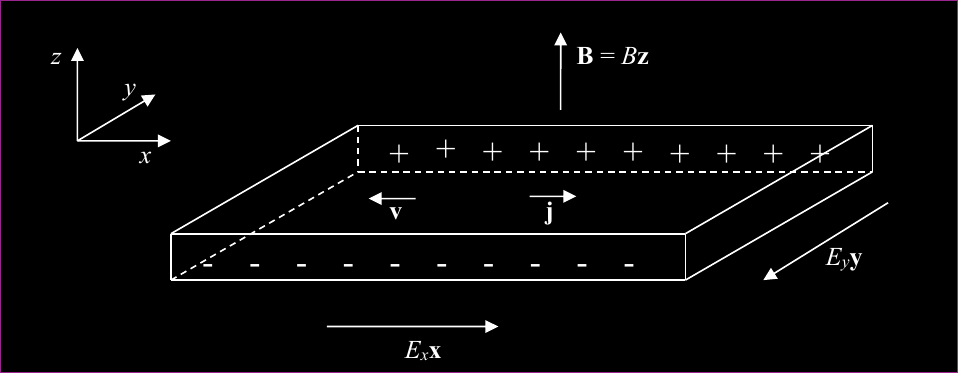
\includegraphics[width=\linewidth]{images/Hall experiment.png}
\end{figure}
  
A geometria do experimento Hall parte do pressuposto que temos dois campos sendo aplicados em nossa amostra, um campo elétrico sendo aplicado na direção +x, $E_x\hat{x}$ e um campo magnético sendo aplicado perpendiculamente, direção z, $\mathbf{B} = Bz$. O campo elétrico $E_x\hat{x}$ faz com que tenhamos uma corrente elétrica nesse sentido, $j$. Como temos um campo magnético sendo aplicado da direção z, ocorre uma defleção dos elétrons por conta da força de Lorentz. Sendo assim, cargas negativas começam a acumular de um lado da amostra. Essa diferença de cargas na parede faz com que surja um campo elétrico na direção $-E_y\hat{y}$, sendo assim, surje uma corrente elétrica, que seria a corrente de Hall.

Analisando esse experimento no regime estacionário, ou seja, quando $\dv{v_y}{t} = 0$, temos então que na direção y:

\begin{equation}
  0 = q(E_y + v_xB) \Implies E_y = -v_xB
\end{equation}

Onde o $E_y$ é justamente o nosso campo Hall. Sabemos que a densidade da corrente é $j = nqv_x$. Substituindo $v_x$ no campo de Hall, obtemos:

\begin{equation}
    E_y = -\frac{j_x}{nq}B 
\end{equation}

E o coeficiente Hall é definido como: 

\begin{equation}
    R_H = \frac{E_y}{j_xB} = - \frac{1}{nq} 
\end{equation}

Em um experimento Hall, conseguimos medir $E_y$ e nós já conhecemos a $j_x$ e $B$, afinal, eles são aplicados de maneira controlada. Sendo assim, podemos calcular o coeficiente Hall e usar a expressão que relaciona ele com a densidade dos portadores de carga:
\begin{equation}
R_H = -\frac{1}{nq} \Implies n = -\frac{1}{R_Hq}
\end{equation}

\item Interprete e explique a dependência da temperatura na densidade de portadores de carga para o Ge dopado tipo-n com diferentes contrações de dopantes $N_d$, figura abaixo.

  \begin{center}
\begin{figure}[htbp]
  \centering
  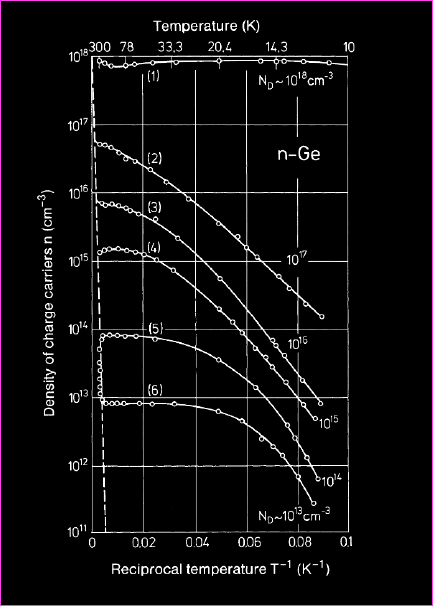
\includegraphics[scale=0.5]{images/Ge dopado.png}
\end{figure}
\end{center}
A primeira coisa que eu notei ao observar a imagem, é que no caso do nosso semicondutor puro, intrínseco, a densidade de portadores delétrons só começa a ser relevante a partir de altas temperatura. Supondo que a função que descreve a densidade dos portadores de elétrons seja contínua, e a "tendência" da função seja a mesma, é possível perceber que a densidade dos portadores de elétrons do semicondutor intrínseco para baixas temperaturas fica praticamente perto de zero, sendo negligenciável se comparado com sua versão dopada. Dessa forma, o nosso semicondutor à baixas temperaturas age basicamente como um isolante. Ao introduzirmos uma dopagem tipo-n no nosso Ge, temos mais elétrons disponíveis. Analisando o impacto da diferentes concentrações de dopantes e temperatura na densidade dos portadores de cargas, é possível notar-se algumas coisas. Primeiro, a é que parecem haver três "regimes" que determinam a densidade dos portadores de carga. Em baixas temperaturas, temos que $n << N_d$, e para baixas concentrações de $N_D$, o crescimento de $n$ com a temperatura parece ocorrer de maneira logarítima, até que chegamos à situação onde $n = N_D$. Nessa situação a variação de temperatura não afeta muito $n$, até que chegamos no regime de altas temperaturas e $n>N_D$. Nesse caso, podemos presumir que a temperatura foi o suficiente para ionizar os átomos, fazendo com que mais elétrons vão para a banda de condução, deixando buracos na banda de valência. É interessante notar que o aumento de concentração de dopantes faz com que o comportamento da função no gráfico $n \times K$ seja cada vez mais linear. Porém, quando chegamos em uma concentração tão alta de dopante, $N_D = 10^{18}$, praticamente a densidade de portadores de cargas é uma constante. Eu pressuponho que isso ocorre pelo fato da quantitade de elementos dopantes serem extremamente maiores do que a quantidade de átomos de Germânio.
  
\item {}
\end{enumerate}


\end{document}

